% ML4H 2026 submission -- Faithful and Fair? Skin-tone equity audit of concept-based dermatology AI
% Compile with pdfLaTeX on Overleaf (search "ML4H 2026" or use the JMLR/PMLR class).
% Needs: jmlr.cls (ships with the ML4H template), ref.bib, and figures/{audit,faithfulness,mitigation}.pdf
\documentclass[pmlr,twocolumn,10pt]{jmlr}

% Submission track. Proceedings is the archival PMLR track (8-page main-content limit,
% excluding references and appendices). The per-concept decomposition lives in the
% appendix to fit that limit. Switch to "findings" for the shorter non-archival version.
\mlhtrack{proceedings}

\newif\iffinal
\finalfalse   % set \finaltrue for the camera-ready version

\iffinal
    \ifmlhneedspmlr
      \jmlrvolume{XXX}
      \jmlryear{2026}
    \fi
    \ifmlhfindings \jmlrproceedings{}{ML4H 2026 - Findings Track}\fi
    \ifmlhdemo     \jmlrproceedings{}{ML4H 2026 - Demo Track}\fi
    \jmlrworkshop{Machine Learning for Health (ML4H) 2026}
\else
    \jmlrproceedings{}{Submitted to ML4H 2026: \mlhtrackname}
    \jmlrworkshop{Machine Learning for Health (ML4H) 2026}
\fi

\urlstyle{same}
\usepackage{booktabs}
\usepackage{siunitx}
\usepackage[switch]{lineno}

\title[Faithful and Fair?]{Faithful and Fair? A Skin-Tone Equity Audit of the
Predictions and Explanations of a Concept-Based Dermatology Model}

\author{Anonymous Author(s)}

\linenumbers

\begin{document}

\maketitle

\ifmlhdemo\else
\begin{abstract}
Skin-tone disparities in dermatology AI are, by now, well documented---but they
are almost always measured on the model's \emph{predictions}. We ask a
different question: is the model's stated clinical \emph{reasoning} equally
sound across skin tones? Using a frozen dermatology vision-language model
(DermLIP) as a concept bottleneck over the 7-point checklist, we run every
comparison with bootstrap confidence intervals and permutation tests so that
small effects are not mistaken for findings. Four results follow. First, on
Derm7pt a soft monotonicity objective makes the concept-to-diagnosis mapping
perfectly intervention-consistent (0.74\,$\rightarrow$\,1.00)---that is,
asserting a melanoma criterion never lowers the predicted melanoma
probability---at no cost to accuracy or melanoma AUROC. Second, the familiar
prediction disparity is large and significant---a light-versus-dark AUROC gap of
0.162 on Fitzpatrick17k ($p<10^{-4}$), reproduced on biopsy-proven DDI (0.75
vs.\ 0.56, disjoint CIs). Third, and new, the \emph{faithfulness} of the
explanation is itself significantly lower on darker skin in-distribution
(monotonicity 0.650 vs.\ 0.603, disjoint 95\% CIs), though this does not reach
significance on the smaller external set. Fourth, a standard worst-group
intervention (Group-DRO) does not close either gap. We read this as early but concrete evidence that
fair predictions are not the same as fair explanations, and that the latter
deserves to be measured directly.
\end{abstract}
\begin{keywords}
algorithmic fairness, dermatology, concept bottleneck models, interpretability,
faithfulness, skin tone, vision-language models
\end{keywords}
\fi

\ifmlhneedsstatements
\paragraph*{Data and Code Availability}
This study is a secondary analysis of three publicly available dermatology
datasets: Derm7pt \citep{kawahara2019sevenpoint}, Fitzpatrick17k
\citep{groh2021evaluating}, and the Diverse Dermatology Images (DDI) set
\citep{daneshjou2022disparities}. Derm7pt and Fitzpatrick17k are openly
downloadable; DDI is available from the Stanford AIMI repository under a data
use agreement. We release all code, prompts, and the cached frozen features
needed to reproduce every number and figure in this paper; an anonymized
repository is linked in the supplementary material for review.

\paragraph*{Institutional Review Board (IRB)}
This work uses previously collected, de-identified, publicly released image
datasets and does not involve any interaction with human subjects or access to
identifiable private information. It therefore does not constitute human
subjects research and did not require IRB approval.
\fi

\section{Introduction}
\label{sec:intro}

That dermatology classifiers work less well on darker skin is one of the more
robust findings in medical imaging fairness. It has been shown for
convolutional networks trained on clinical photographs
\citep{groh2021evaluating}, for commercial and academic models evaluated on
biopsy-proven images \citep{daneshjou2022disparities}, and across a range of
architectures and tone definitions \citep{kinyanjui2020fairness}. The community
response has largely been to measure and try to reduce the gap in the model's
\emph{output}---its accuracy, sensitivity, or AUROC by skin-tone group.

We think there is a second question hiding underneath the first, and it has
received far less attention. Modern high-stakes advice from a model is expected
to come with a reason, and there is a long argument that in medicine the reason
should be interpretable by construction rather than reconstructed after the fact
\citep{rudin2019stop}. A concept bottleneck model is one clean way to get such a
reason: the network first predicts human-defined clinical concepts, and the
diagnosis is then a function of those concepts alone \citep{koh2020concept}.
When we build such a model for skin lesions, a fairness question appears that
prediction-level audits cannot see. Even if two patients received equally
\emph{accurate} predictions, are the \emph{explanations} equally
\emph{faithful}---does the stated reasoning actually drive the diagnosis as
reliably for a patient with Fitzpatrick type VI skin as for type II? Faithfulness
in this sense---whether the explanation reflects the computation the model
actually performs \citep{jacovi2020towards}---is not guaranteed by accuracy, and
post-hoc explanations are known to fail sanity checks that faithful ones should
pass \citep{adebayo2018sanity}.

This paper is an attempt to measure that directly, carefully, and honestly. We
use a frozen dermatology-specific vision-language model, DermLIP, as the
backbone, read out the seven criteria of the 7-point melanoma checklist
\citep{argenziano1998epiluminescence} as concepts, and train small heads that
map concepts to a malignancy decision. \figureref{fig:pipeline} shows the whole
pipeline at a glance. Because the backbone is frozen and the
heads are tiny, the whole study runs on a single free-tier GPU for the one-time
image encoding and on a laptop CPU for everything else, which we note only
because it makes the work easy to reproduce and extend.

Our contributions are as follows.
\begin{itemize}
  \item \textbf{A faithfulness objective that is free.} On Derm7pt, where the
  concepts have ground truth, a soft \emph{monotonicity} penalty---a criterion
  for melanoma may never decrease the predicted probability of
  melanoma---raises intervention consistency from 0.74 to a perfect 1.00 while
  leaving balanced accuracy and melanoma AUROC unchanged
  (\sectionref{sec:h1}). Rewarding exact agreement with the discrete checklist
  \emph{score}, by contrast, was counterproductive in our ablations.
  \item \textbf{A powered, significant prediction audit.} The light-versus-dark
  malignancy AUROC gap is 0.162 (95\% CI $[0.071, 0.262]$, permutation
  $p<10^{-4}$) on Fitzpatrick17k, and reproduces zero-shot on biopsy-proven DDI
  (0.752 vs.\ 0.564, disjoint CIs) (\sectionref{sec:audit}).
  \item \textbf{First evidence that explanation faithfulness is itself
  inequitable.} In-distribution, monotonicity is significantly lower on darker
  skin (0.650 vs.\ 0.603, disjoint 95\% CIs). We report this as a real but
  preliminary result: it does not reach significance on the smaller external
  set, and both values sit on a weak zero-shot concept substrate
  (\sectionref{sec:h3}).
  \item \textbf{An honest negative.} Group-DRO, the standard worst-group
  training method, does not significantly raise worst-group AUROC in either
  setting, and cross-dataset transfer collapses toward chance
  (\sectionref{sec:h2}).
\end{itemize}

We want to be clear about scope. None of these results, on their own, is a
solved problem, and the faithfulness gap in particular is a first look rather
than a settled fact. The point of the paper is to show that the question is
measurable and that the answer, so far, is not reassuring.

\section{Related Work}
\label{sec:related}

\paragraph{Skin-tone fairness in dermatology AI.}
\citet{esteva2017dermatologist} brought dermatologist-level classification into
reach, but subsequent audits found that performance is uneven across skin
tones. \citet{groh2021evaluating} released Fitzpatrick17k and showed that models
trained on it degrade on the darkest tones; \citet{daneshjou2022disparities}
assembled DDI, a small but biopsy-proven and tone-balanced set, and reported
sharp drops on type V--VI skin for several models; \citet{kinyanjui2020fairness}
studied the effect systematically at MICCAI. Our prediction-level results
reproduce this literature on a newer, dermatology-specific vision-language
backbone. Our departure is to ask the same fairness question about the
explanation rather than only the label.

\paragraph{Interpretability and faithfulness.}
\citet{rudin2019stop} argues for models that are interpretable by design in
high-stakes settings; concept bottleneck models \citep{koh2020concept} and their
post-hoc variants \citep{yuksekgonul2023posthoc} are a practical realization,
and CLIP-style backbones \citep{radford2021learning} make it easy to read
concepts out of a frozen encoder. Faithfulness---whether an explanation
reflects the model's actual computation---has a careful definition in NLP
\citep{jacovi2020towards}, and the fragility of post-hoc saliency
\citep{adebayo2018sanity} is a large part of why concept bottlenecks are
attractive. To our knowledge, faithfulness has not previously been audited as a
\emph{fairness} quantity across patient subgroups.

\paragraph{Group robustness.}
Group-DRO \citep{sagawa2020distributionally} optimizes the worst group's loss
and is the default reach-for method when a subgroup underperforms. We use it
as our mitigation baseline; the fact that it does not help here is itself worth
recording.

\section{Method}
\label{sec:method}

\begin{figure*}[t]
\floatconts
  {fig:pipeline}
  {\caption{The pipeline in one picture. A frozen dermatology encoder (DermLIP)
  turns a lesion image into seven concept scores---one per 7-point-checklist
  criterion---by comparing the image to ``present'' and ``absent'' text prompts.
  A small trained head maps those seven numbers to a malignancy probability, so
  the concepts are the only thing standing between image and decision. We test
  \emph{faithfulness} by intervening on a concept (force a melanoma criterion on;
  a faithful model must not lower the predicted risk), and we \emph{audit} every
  quantity separately for light, mid, and dark skin.}}
  {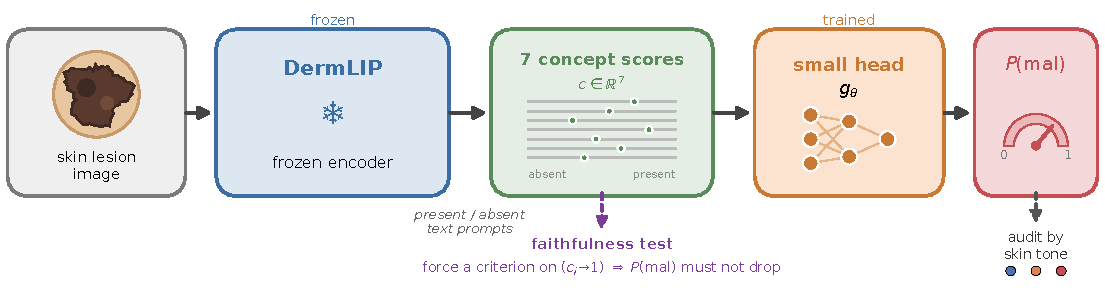
\includegraphics[width=\linewidth]{figures/pipeline}}
\end{figure*}

\paragraph{Backbone and concepts.}
We use DermLIP ViT-B/16 \citep{dermlip2025}, a CLIP-style model
\citep{radford2021learning} trained on a large dermatology image-text corpus,
and keep it entirely frozen. For each image we cache the image embedding and,
for each of the seven checklist criteria, a concept score obtained by comparing
the image embedding to the text embeddings of a ``present'' and ``absent''
prompt. On Derm7pt, which carries concept ground truth, we can also train
supervised concept probes; on the clinical-photo datasets (Fitzpatrick17k, DDI)
no concept labels exist, so we use these prompt-based scores directly---%
\emph{zero-shot}, meaning no concept labels are ever used to fit them. We chose
DermLIP over the general biomedical BiomedCLIP \citep{zhang2023biomedclip}
because it is dermatology-specific; BiomedCLIP is kept only as a sanity baseline.

\paragraph{Concept bottleneck.}
Let $c \in \mathbb{R}^{7}$ be the vector of concept scores for an image. A small
two-layer network $g_\theta$ maps $c$ to a malignancy logit,
$\hat{y} = \sigma(g_\theta(c))$, with $\sigma$ the logistic function. Because $g_\theta$ sees only $c$, the concept
vector is the entire interface between image and decision, which is what makes
an intervention on a concept meaningful.

\paragraph{A directional faithfulness objective.}
We call the model faithful, in the narrow sense we can test, if forcing a
melanoma criterion \emph{on} never lowers the predicted probability of
malignancy. For concept $i$ and input $c$, write $c^{i\rightarrow 1}$ and
$c^{i\rightarrow 0}$ for $c$ with coordinate $i$ set to present and absent. We
measure \emph{intervention consistency} (equivalently, monotonicity) as the
fraction of (sample, concept) pairs for which
$\hat{y}(c^{i\rightarrow 1}) \ge \hat{y}(c^{i\rightarrow 0})$, and add a soft
hinge penalty on violations to the training loss. This is a differentiable
relaxation of a monotonic network \citep{sill1998monotonic}. Crucially, we
found that a competing objective---rewarding the head for reproducing the
discrete checklist \emph{score} of ``$\ge 3$ points $\Rightarrow$ suspicious''
\citep{argenziano1998epiluminescence}---caps the model at the rule's quality and
degrades melanoma sensitivity, so we do not use it.

\paragraph{Equity training.}
For the fairness experiments we compare standard empirical risk minimization
(ERM) against Group-DRO \citep{sagawa2020distributionally} over three skin-tone
groups (light = Fitzpatrick I--II, mid = III--IV, dark = V--VI), which reweights
the loss toward the worst-performing group online.

\paragraph{Statistics.}
Every group AUROC---the probability the model scores a random malignant lesion
above a random benign one, where 0.5 is chance---is reported with a percentile
bootstrap 95\% confidence interval \citep{efron1994introduction}. For the central disparity claim we add a
\emph{permutation test}: we pool the light and dark samples, repeatedly shuffle
the group labels, and recompute the AUROC gap to build a null distribution. For
the mitigation claim we use a \emph{paired} bootstrap of the ERM$-$Group-DRO
difference in worst-group AUROC, so a CI that contains zero is read as no
significant effect. Faithfulness gaps are gated the same way, using bootstrap
CIs on the per-group monotonicity.

\section{Experimental Setup}
\label{sec:setup}

\paragraph{Datasets.}
Derm7pt \citep{kawahara2019sevenpoint} ($\approx$\,1{,}011 cases) provides the
concept ground truth for the faithfulness experiment. For the audit we use
Fitzpatrick17k \citep{groh2021evaluating} for scale and tone diversity and DDI
\citep{daneshjou2022disparities} as an external, biopsy-proven test set;
\tableref{tab:cohort} gives their composition. Two features of the data shape
everything downstream. First, malignant lesions on dark skin are scarce---208 in
all of Fitzpatrick17k, of which only 39 fall in its test split, and 48 in
DDI---which is what widens the dark-skin confidence intervals and leaves the
external comparison underpowered. Second, we map each dataset's tone annotation
onto three groups (light = Fitzpatrick I--II, mid = III--IV, dark = V--VI);
Fitzpatrick17k tone is estimated from the image rather than assigned by a
clinician, a limitation we return to. We drop the 565 Fitzpatrick17k images with
unusable tone labels, leaving 16{,}012 of the 16{,}577 cached images for the
tone analysis.

\begin{table}[htbp]
\floatconts
  {tab:cohort}
  {\caption{Cohort composition after tone mapping (malignant counts in
  parentheses). The scarcity of malignant dark-skin lesions---39 in the
  Fitzpatrick17k test split, 48 in DDI---is the main limit on statistical power
  for the dark group.}}
  {\small
  \begin{tabular}{lrr}
  \toprule
   & Fitzpatrick17k & DDI (ext.) \\
   & images (malig.) & images (malig.) \\
  \midrule
  light  & 7{,}755 (1{,}195) & 208 (49) \\
  mid    & 6{,}089 (757)     & 241 (74) \\
  dark   & 2{,}168 (208)     & 207 (48) \\
  \midrule
  total  & 16{,}012 (2{,}160) & 656 (171) \\
  \bottomrule
  \end{tabular}}
\end{table}

\paragraph{Protocol.}
Images are encoded once with the frozen backbone and cached. For the audit we
train the concept-to-malignancy head on the Fitzpatrick17k training split and
evaluate both in-distribution (its test split) and externally (all of DDI).
Heads are two-layer MLPs (hidden width 16) trained for 1{,}500 steps with Adam;
we ensemble three seeds and report ensembled probabilities. Because clinical
photographs have no concept ground truth, the audit uses zero-shot concepts;
the Derm7pt faithfulness experiment uses supervised probes.

\paragraph{The representation already encodes skin tone.}
Before any head is trained, skin tone is easy to read straight off the frozen
embedding: a linear probe (a linear classifier on the 512-dimensional frozen
features) recovers the three tone groups at 0.71 accuracy, well above the 0.48
majority-class baseline, with one-versus-rest AUROCs of 0.88, 0.78, and 0.91 for
light, mid, and dark. The protected attribute is thus baked into the
representation every downstream head consumes---worth keeping in mind for the
disparities that follow, since ``just ignore skin tone'' is not an option the
model actually has.

\section{Results}

\subsection{A faithfulness objective at no accuracy cost}
\label{sec:h1}

\tableref{tab:h1} summarizes the Derm7pt experiment. An unrestricted linear
probe on the frozen embedding reaches 0.877 melanoma AUROC; routing the decision
through the seven concepts costs essentially nothing on melanoma. Training with
correctness alone leaves the concept-to-diagnosis map only partly
faithful---intervention consistency is 0.74, meaning that about a quarter of the
time, asserting a melanoma criterion does not increase the predicted
probability of melanoma. Adding the monotonicity objective removes every such
violation (consistency 1.00) and, if anything, nudges accuracy up (0.797 to
0.830) with melanoma AUROC unchanged at 0.87. The explanation becomes
directionally trustworthy for free. We read the earlier, failed rule-matching
variant as the reason: faithfulness is best encouraged by constraining the
\emph{direction} of the concept's effect, not by forcing the head to imitate a
hand-set threshold.

\begin{table}[htbp]
\floatconts
  {tab:h1}
  {\caption{Faithfulness on Derm7pt (5-class head, 3 seeds). Adding the
  monotonicity objective makes the concept$\rightarrow$diagnosis map perfectly
  intervention-consistent at no cost to accuracy or melanoma AUROC.}}
  {\small\setlength{\tabcolsep}{4pt}%
  \resizebox{\ifdim\width>\columnwidth \columnwidth\else\width\fi}{!}{%
  \begin{tabular}{lccc}
  \toprule
   & Acc. & Mel.\ AUC & Cons. \\
  \midrule
  Linear probe (ref.) & 0.846 & 0.877 & --- \\
  Bottleneck (corr.)  & 0.797 & 0.873 & 0.74 \\
  \;+ monotonicity    & 0.830 & 0.875 & \textbf{1.00} \\
  \bottomrule
  \end{tabular}}}
\end{table}

\subsection{The prediction disparity is large and real}
\label{sec:audit}

\figureref{fig:audit} is the headline audit. On Fitzpatrick17k the
concept-bottleneck malignancy AUROC falls monotonically with skin tone, from
0.841 $[0.810, 0.871]$ on light skin to 0.679 $[0.594, 0.765]$ on dark skin. The
light-versus-dark gap is 0.162, with a bootstrap 95\% CI of $[0.071, 0.262]$
that excludes zero, and a permutation test rejects the null of no disparity at
$p<10^{-4}$. The same pattern appears zero-shot on biopsy-proven DDI (light
0.752 $[0.674, 0.826]$ vs.\ dark 0.564 $[0.467, 0.664]$), where the dark-group
CI reaches down toward chance. Two datasets, two readout methods, the same
direction: this is not a sampling artifact.

\begin{figure*}[t]
\floatconts
  {fig:audit}
  {\caption{Malignancy AUROC by skin-tone group with bootstrap 95\% CIs.
  \emph{Left}: concept bottleneck trained and tested on Fitzpatrick17k
  (light--dark gap 0.162, permutation $p<10^{-4}$). \emph{Right}: DermLIP
  zero-shot on biopsy-proven DDI (light and dark CIs disjoint). The disparity
  reproduces across datasets and readout methods.}}
  {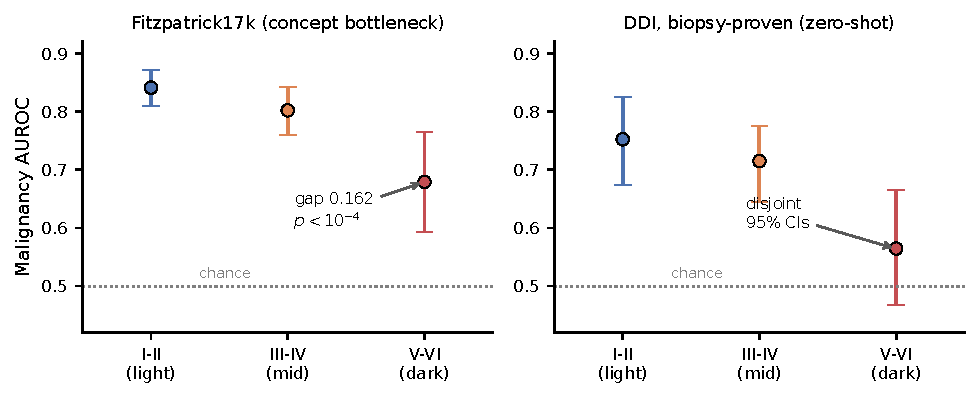
\includegraphics[width=\linewidth]{figures/audit}}
\end{figure*}

\subsection{Explanation faithfulness is lower on darker skin---in-distribution}
\label{sec:h3}

The question the paper is really about is in \figureref{fig:faith}. On the
Fitzpatrick17k test set, the per-group monotonicity of the trained bottleneck
declines with tone---light 0.650 $[0.643, 0.658]$, mid 0.629 $[0.621, 0.637]$,
dark 0.603 $[0.589, 0.618]$---and the light and dark confidence intervals are
disjoint. Within this distribution, then, the explanation is measurably less
faithful for darker skin, not just less accurate. We did not assume this would
be significant, and were somewhat surprised that it survived the bootstrap.

Two honest caveats keep us from overclaiming. First, on the smaller external DDI
set the same comparison is not significant (light 0.662 $[0.651, 0.674]$ vs.\
dark 0.648 $[0.634, 0.661]$, overlapping), so we cannot yet say the effect
transfers to biopsy-proven images. Second, the absolute monotonicity is only
$\approx$\,0.6 for every group, because zero-shot concepts on clinical
photographs are weak; a gap between two mediocre explainers is real but should
be read as a signal to investigate, not as a verdict. We therefore present the
faithfulness gap as the first concrete evidence that fairness of explanations is
a distinct and measurable problem, and leave its full characterization to
future work (\sectionref{sec:discussion}). A per-concept, per-tone decomposition
(Appendix~\ref{sec:mech}) localizes the gap to weak, unevenly extracted concepts
and a head that inherits their flaws, rather than to any single criterion.

\begin{figure}[htbp]
\floatconts
  {fig:faith}
  {\caption{Explanation faithfulness (intervention consistency / monotonicity)
  by skin tone, with bootstrap 95\% CIs. In-distribution (Fitzpatrick17k) the
  light and dark CIs are disjoint---faithfulness is significantly lower on
  darker skin. On the smaller external DDI set the gap is not significant.}}
  {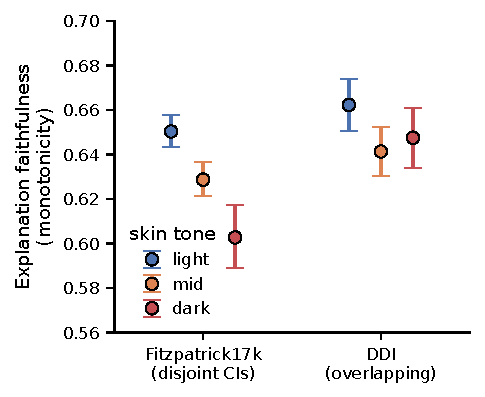
\includegraphics[width=0.85\linewidth]{figures/faithfulness}}
\end{figure}

\subsection{Group-DRO does not close the gap}
\label{sec:h2}

If the disparity is real, the obvious next move is to train for it.
\figureref{fig:mitig} shows what happened when we did. Group-DRO changes the
worst-group (dark) AUROC on Fitzpatrick17k by $+0.014$, with a paired-bootstrap
95\% CI of $[-0.011, 0.041]$ that comfortably contains zero; on external DDI the
change is $-0.034$ $[-0.074, 0.001]$, if anything slightly worse. The
light--dark gap is essentially unmoved. Separately, a bottleneck trained on
Fitzpatrick17k and applied to DDI collapses toward chance (dark AUROC 0.461
$[0.370, 0.551]$), a reminder that the domain shift from web/clinical
photographs to biopsy-proven images is severe. We report both as negative
results: the standard worst-group intervention is not a fix here, and
cross-dataset generalization cannot be assumed.

\begin{figure}[htbp]
\floatconts
  {fig:mitig}
  {\caption{ERM vs.\ Group-DRO malignancy AUROC by skin tone on Fitzpatrick17k
  (bootstrap 95\% CIs). The worst-group (dark) AUROC changes by only $+0.014$
  $[-0.011, 0.041]$, not significant, and the light--dark gap is essentially
  unmoved.}}
  {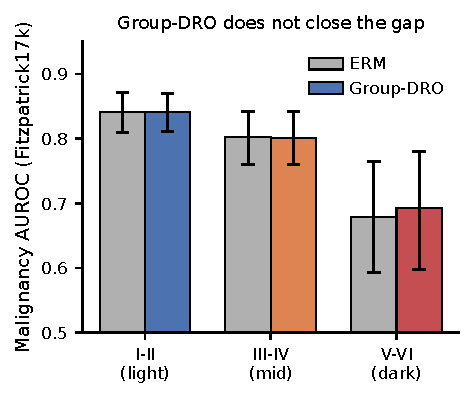
\includegraphics[width=0.85\linewidth]{figures/mitigation}}
\end{figure}

\section{Discussion}
\label{sec:discussion}

The cleanest way to state what we found is by what it rules out. Fair
predictions do not imply fair explanations: on Fitzpatrick17k the model's
reasoning is significantly less faithful for darker skin even though every group
is scored by the same head. And the reflexive fix does not work: Group-DRO,
which is designed precisely to lift a failing subgroup, produces no significant
improvement in either accuracy or---by extension---the machinery that would have
to improve for the explanation to become fair.

A tempting misreading is that the faithfulness gap is simply the accuracy gap in
disguise. We do not think so, because the two are computed differently---AUROC
compares malignant against benign within a group, while monotonicity asks
whether concept interventions move the prediction in the clinically correct
direction, a property of the head's response surface rather than of its ranking.
The per-concept decomposition in \sectionref{sec:mech} lets us localize the
gap---to weak, unevenly extracted concepts and a head that inherits their
flaws---but not cleanly attribute it, because backbone and head failures are
coupled. Untangling them is exactly the work we think should come next.

\paragraph{Limitations.}
Several, stated plainly. The faithfulness gap is significant only
in-distribution; the external set is small and its comparison is not
significant. The concept scores on clinical photographs are zero-shot and weak,
so the monotonicity values are low in absolute terms. Fitzpatrick17k tone is
estimated from the image, not assigned by a clinician, and the dataset has known
label-quality issues. We study a single backbone and a single faithfulness
metric. And the ``policy'' framing we experimented with early on reduces, for
seven cached features, to a shallow optimization detail, so we do not claim it
as a contribution.

\paragraph{What a convincing version would need.}
We see a clear path from this preliminary result to a robust one, and record it
so others (or we) can follow it. It has three parts. \emph{(i)~Robustness}:
replicate the faithfulness gap across more than one backbone (e.g.,
BiomedCLIP and a larger dermatology encoder), more than one faithfulness metric,
and---critically---on an external set large enough to have power, so the effect
is not a single-model, in-distribution artifact. \emph{(ii)~Mechanism}: our per-concept
decomposition (\sectionref{sec:mech}) is a first descriptive step, but it cannot
separate whether darker-skin explanations are less faithful because the concepts
themselves are noisier there or because the head's response surface is genuinely
less monotone in that region of concept space---the two are coupled, and
breaking that coupling needs concept ground truth on diverse clinical images,
which does not currently exist at scale. \emph{(iii)~A mitigation that actually works}: since Group-DRO does
not, a method that equalizes faithfulness---for instance a per-group
monotonicity penalty or concept-space reweighting---would turn the audit into a
solution. We flag this as the natural extension toward a full methods paper; the
present work establishes that the problem is real enough to be worth it.

\section{Conclusion}

Auditing dermatology AI for skin-tone fairness usually stops at the prediction.
When we look one level down, at whether the model's concept-based reasoning is
equally faithful across tones, we find---carefully, with confidence intervals
and permutation tests---that it is not, at least in-distribution, and that the
standard fairness fix does not repair it. The faithfulness gap is preliminary
and we have tried not to oversell it. But it is measurable, and we think that
alone is a reason to start measuring it.

% Acknowledgments appear only in the camera-ready version.
% \acks{...}

\bibliography{ref}

\appendix

\section{Per-concept decomposition of the faithfulness gap}
\label{sec:mech}

\begin{figure*}[t]
\floatconts
  {fig:diag}
  {\caption{Decomposing the faithfulness gap on Fitzpatrick17k, per concept and
  per tone. \emph{(a)}~Backbone: each criterion's zero-shot malignancy AUROC
  within a tone group---blue-whitish veil separates best, atypical vascular is
  below chance for all groups, and the informative concepts (pigment network,
  streaks) lose signal on darker skin. \emph{(b)}~Head: the faithfulness
  violation rate per criterion---the fraction of lesions for which forcing the
  criterion \emph{on} lowers predicted malignancy. Violations concentrate on the
  concept the backbone extracts as anti-signal (atypical vascular) and rise with
  darker tone. The two panels are coupled: the head faithfully inherits the
  backbone's concept flaws.}}
  {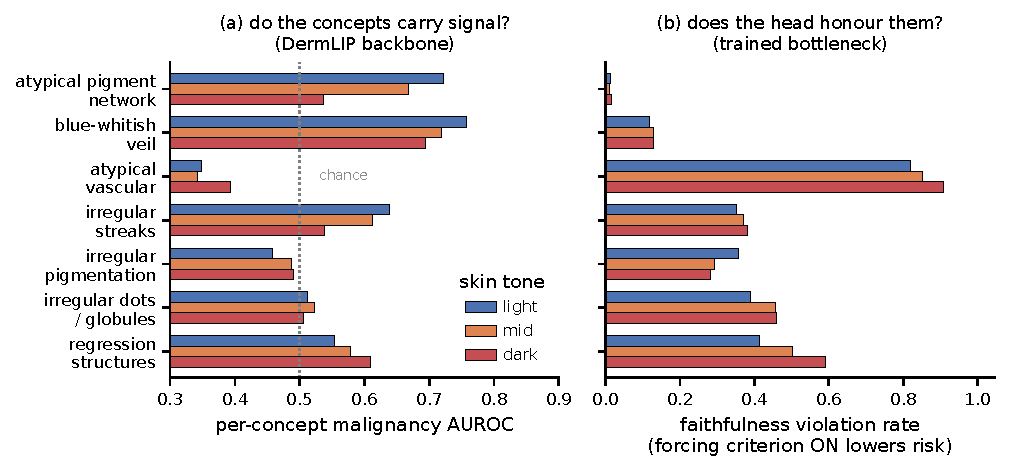
\includegraphics[width=\linewidth]{figures/diagnostic}}
\end{figure*}

\figureref{fig:diag} breaks the aggregate monotonicity number apart on the
Fitzpatrick17k test set---which of the seven criteria misbehave, and for whom.
The left panel asks whether each concept, as DermLIP reads it zero-shot,
even separates malignant from benign: the concepts are strikingly uneven.
Blue-whitish veil is the one dependable signal (AUROC $\approx 0.76$); atypical
vascular structures sit \emph{below} chance for every tone group ($\approx
0.35$), meaning DermLIP's score for that criterion is if anything
anti-correlated with malignancy; and the criteria that do carry signal decay on
darker skin, most sharply the atypical pigment network (0.72 on light skin to
0.54---near chance---on dark). The right panel then asks whether the trained
head honours each criterion directionally. Violations are dominated by exactly
the concept the backbone gets backwards: because atypical vascular is
anti-correlated with the label, the head rationally learns a negative weight on
it, so forcing it \emph{on} lowers predicted risk 82--91\% of the time. Two
things are worth naming honestly here. First, the panels are coupled, not
independent---a concept the backbone extracts as anti-signal mechanically forces
a data-faithful head into rule-violation, which is the same
correctness-versus-faithfulness tension we saw on Derm7pt
(\sectionref{sec:h1}), now visible per concept. Second, the tone gradient runs
through \emph{both} panels: separability is lowest on dark skin and the
per-concept violation rate is highest there (regression structures, for example,
climb from 0.41 to 0.59 light-to-dark). Averaged over concepts the violation
rates are 0.35 / 0.37 / 0.40 for light / mid / dark, which is exactly the
complement of the monotonicity in \figureref{fig:faith}. So the faithfulness gap
does not live in one place we can excise; it is distributed across weak, unevenly
extracted concepts and a head that faithfully inherits their flaws. That is a
localization, not yet a mechanism, and we treat it as such.

\end{document}
